% !TEX program = xelatex
% Adapted from TDReportTemplate_CN_TITLE.tex supplied by the user.
\RequirePackage[T1]{fontenc}
\documentclass[12pt,journal,onecolumn,a4paper]{IEEEtran}
\usepackage[UTF8,fontset=fandol,scheme=chinese]{ctex}
\setmainfont{texgyretermes}[Extension=.otf,UprightFont=*-regular,BoldFont=*-bold,ItalicFont=*-italic,BoldItalicFont=*-bolditalic]
\usepackage{graphicx,amsmath,amssymb,bm,booktabs,tabularx,longtable,array}
\usepackage{indentfirst,placeins,caption,microtype,xcolor,listings,enumitem,xurl,float,needspace,etoolbox}
\usepackage[numbers,square,sort&compress]{natbib}
\usepackage[unicode,colorlinks=true,linkcolor=blue,citecolor=blue,urlcolor=blue]{hyperref}
\usepackage{float}
\hypersetup{pdftitle={TableLab：基于本地字段检索的中文表格问答与预测},pdfauthor={郑嘉诚},pdfsubject={天津大学机器学习与人工智能课程报告}}
\captionsetup{hypcap=false,font=small,labelfont=bf,labelsep=quad,skip=5pt}
\setlength{\parindent}{2\ccwd}
\setlength{\parskip}{3pt plus .5pt minus .3pt}
\emergencystretch=2em
% Allow figures and tables to share pages with text.
\renewcommand{\topfraction}{.9}
\renewcommand{\bottomfraction}{.85}
\renewcommand{\textfraction}{.08}
\renewcommand{\floatpagefraction}{.85}
\setcounter{topnumber}{3}
\setcounter{bottomnumber}{2}
\setcounter{totalnumber}{4}
\raggedbottom
\setcounter{tocdepth}{1}
\makeatletter
\renewcommand*\l@section{\@dottedtocline{1}{0em}{4.5em}}
\makeatother
\newcommand{\field}[1]{\texttt{#1}}
\newcommand{\T}{\mathcal{T}}\newcommand{\V}{\mathcal{V}}
\newcommand{\tabnote}[1]{\par\vspace{2pt}\begin{minipage}{\linewidth}\footnotesize #1\end{minipage}}
\newcolumntype{Y}{>{\raggedright\arraybackslash}X}
\newcommand{\inlinetab}[1]{\begin{table}[!htbp]\centering\small #1\end{table}}
\definecolor{InkBlue}{HTML}{184E80}
\newcommand{\code}[1]{\nolinkurl{#1}}
\newcommand{\Train}{\T}\newcommand{\Valid}{\V}
\newcommand{\Ind}{\mathbf 1}
\newcommand{\source}[1]{\par{\footnotesize\raggedright\noindent 计算记录：#1\par}}
\lstset{basicstyle=\ttfamily\small,breaklines=true,columns=fullflexible,keepspaces=true,frame=lines,rulecolor=\color{InkBlue},showstringspaces=false,aboveskip=8pt,belowskip=8pt}
\begin{document}
\begin{titlepage}
\centering
\vspace*{.5cm}
\includegraphics[width=7cm]{logo/TDFonts.pdf}\par
\vspace{1.4cm}
{\fontsize{22}{32}\selectfont\bfseries
TableLab：基于本地字段检索的\\中文表格问答与预测\par}
\vspace{.5cm}
{\large 机器学习课程报告\par}
\vspace{1.2cm}
\includegraphics[width=5.5cm]{logo/TDLogo.pdf}\par
\vfill
{\songti\fontsize{16}{24}\selectfont\bfseries
\renewcommand{\arraystretch}{1.1}
\begin{tabular}{cl}
学\quad 院： & 马寅初经济学院\\\cline{2-2}
专\quad 业： & 应用经济学\\\cline{2-2}
姓\quad 名： & 郑嘉诚\\\cline{2-2}
学\quad 号： & 2026209004\\\cline{2-2}
\end{tabular}\par}
\vspace{.6cm}
{\fontsize{14}{20}\selectfont \today \par}
\vspace*{.5cm}
\thispagestyle{empty}
\end{titlepage}
\setcounter{page}{1}
\title{\textbf{TableLab：基于本地字段检索的\\中文表格问答与预测}}
\author{\href{https://karcen.github.io/}{郑嘉诚}\\马寅初经济学院\quad 应用经济学\quad 2026209004}
\markboth{天津大学机器学习与人工智能课程作业}{郑嘉诚：TableLab}
\maketitle
\patchcmd{\section}{\centering}{\raggedright}{}{}
\patchcmd{\section}{\normalsize}{\large\bfseries}{}{}
\patchcmd{\section}{\scshape}{\relax}{}{}
\begin{abstract}
TableLab 在本地检索字段说明，通过 DeepSeek API 生成分析方案，再由本机程序完成统计与模型训练。字段检索检查限于 16 道固定题，其中 15 道含英文字段名；DeepSeek API 的方案生成质量尚未评价。本文用房价、收入分类、NBA 得分和学生成绩四个任务比较九种预设方法，并对森林与梯度提升分别进行网格和 TPE 搜索。外层三折评价训练流程，内层三折选择参数；训练与验证曲线检查拟合差距，SHAP 和重新调参的特征组消融检查模型依赖。房价的较小平均 RMSE 为 32,338.23 美元，来自提升树＋网格；收入分类中，提升树＋网格的 AUC 为 0.8913。NBA 得分由随机森林取得较小平均误差（5.698 分），学生成绩则是 Ridge（13.545 分）。各任务的较优方法与搜索收益不同，解释和消融结果也需结合字段之间的替代关系判断。
\end{abstract}
\renewcommand{\IEEEkeywordsname}{关键词}
\begin{IEEEkeywords}表格问答；嵌套交叉验证；超参数搜索；SHAP；消融实验\end{IEEEkeywords}
\clearpage\tableofcontents\clearpage
\section{研究问题}


房价表有 81 列。用户问“CollgCr 社区的平均成交价是多少”，实际只需要两列：社区和成交价。先按社区筛选，再给剩下的成交价求平均。如果把所有社区都算进去，程序仍能给出一个均价，但它回答了另一个问题。预测还多一项选择。要估算一套房屋的价格，必须先说明估价时知道哪些房屋属性。

表格问答有几种做法。\citet{herzig2020} 提出的 TaPas 从表中选择单元格，再对所选数值求和、计数或取平均。另一类方法在生成答案前先查资料。\citet{lewis2020} 把这一做法称为检索增强生成（RAG）。本文把检索用于字段说明。检索器查找“成交价”对应哪一列，计算程序读取该列中符合条件的全部记录。这种分工也适合预测任务：检索器查找用户指定的变量，统计程序用这些变量重新拟合模型。

本文分别检查字段检索和模型预测。检索实验记录所需字段在返回结果中的排名。预测实验在同一批验证记录上比较不同输入变量和算法的误差。选列和计算各有可能出错：即使均值算对了，选错列也会答非所问。因此两项实验分别报告。


本文在原固定参数复核之外，比较多类模型及两种超参数搜索，检查训练误差与验证误差的分离，并用字段贡献和重新训练的消融分析预测依据。
\section{结果}
\input{research_results}
\subsection{原单次划分的计算复核}

16 道固定题在四份数据中各占 4 道。每题指定一条应当返回的字段或方法说明，再记录它的排名。15 道题的目标说明排在第一位。余下一题问“\field{player\_name} 是唯一球员身份吗？”。检索器先返回身高说明，再返回姓名说明。因此前六位命中 16 次，平均倒数排名为 $(15+1/2)/16=0.96875$。题库中 15 道题直接写出了目标英文字段名。这组排名反映了这些固定问法下的字段查找结果。自由中文提问与 API 方案质量的后续评价办法见附录~\ref{app:qa-evaluation}。

\subsubsection{房价预测}
房价实验比较两组输入变量。一组使用面积和整体质量，另一组再加入四个变量。按行号核对后，两组使用相同的 1,168 条训练记录和 292 条验证记录。
\inlinetab{\captionof{table}{相同的 292 套房屋，不同的估价方法}\label{tab:houses}
\begin{tabular}{@{}lrr@{}}\toprule
输入变量 & 线性回归 RMSE（美元） & 随机森林 RMSE（美元）\\\midrule
面积、整体质量 & 44,159.60 & 39,205.81\\
再加建成年份、地下室面积、车位数、社区 & 36,461.68 & 33,611.50\\\bottomrule
\end{tabular}
\tabnote{注：给每套房屋都预测训练均价时，RMSE 为 87,619.03 美元。两字段结果来自演示计算，六字段结果来自固定基准实验。两组均有逐条验证预测。}}

加入四个变量后，两种模型的误差都下降。即使用线性回归，六个变量算出的 RMSE 也比两变量随机森林低约 2,744 美元。这说明输入变量会影响算法之间的比较。表~\ref{tab:houses} 记录的是同时加入四个变量后的变化，各变量的单独作用需要另做比较。

六变量线性回归的 MAE 为 22,339.33 美元，随机森林为 20,019.09 美元。用一条验证记录可以直接看出误差的含义。编号 893 的房屋成交价为 154,500 美元，线性回归估价为 141,984.82 美元，低估 12,515.18 美元。计算 MAE 时，这套房屋贡献 12,515.18 美元的绝对误差。计算 RMSE 时，这项误差先取平方。

另一次实验把 2010 年成交的 175 套房屋整年留出，用 2006 至 2009 年的 1,285 套拟合模型。六字段线性回归和森林的 RMSE 分别为 35,008.88 和 30,310.72 美元。森林在两种划分中都取得较小误差。两种划分使用不同的验证房屋，因此分别比较各自的模型误差。

\subsubsection{收入分类}
验证集的 6,512 条记录中有 1,568 个正例。图~\ref{fig:roc} 比较两种模型在不同阈值下的分类结果。纵轴是在实际高收入者中判对的比例。横轴是在其余人中误判为高收入的比例。曲线下面积（AUC）可以理解为，从验证集各取一条正例和负例时，模型给正例更高分的比例；并列分数计作一半。随机森林的 AUC 为 0.8905，逻辑回归为 0.8839。
\begin{figure}[!htbp]\centering
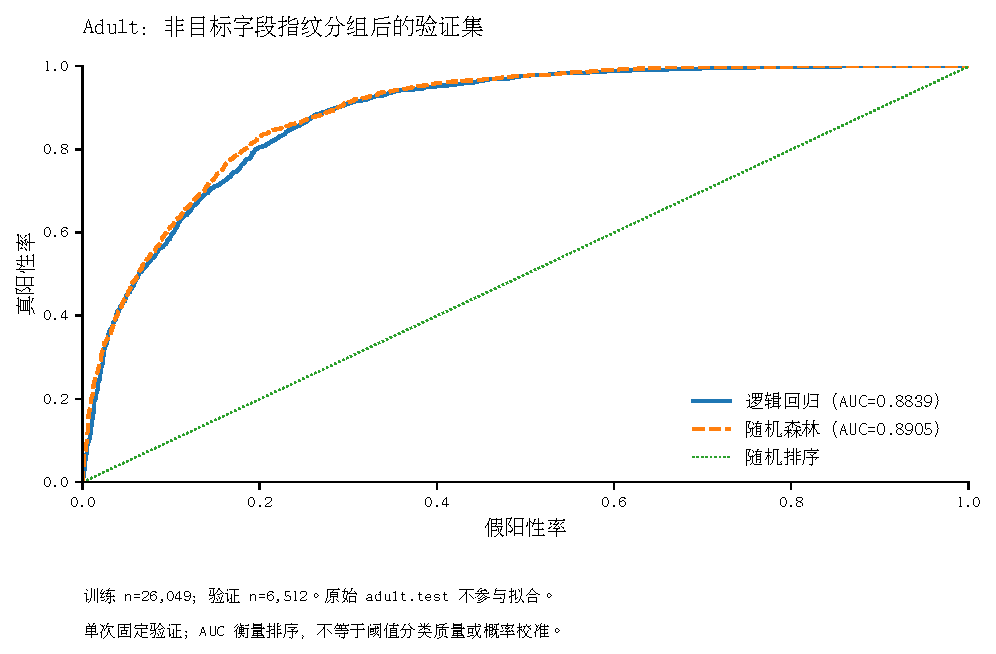
\includegraphics[trim=0 49bp 0 21bp,clip,width=.77\linewidth]{figures/adult_roc.pdf}
\caption{Adult 收入分类的 ROC 曲线。每个阈值对应一个点。斜虚线给出随机排序的参照。}\label{fig:roc}
\end{figure}

固定阈值后，可以直接数出多少人被分错。表~\ref{tab:adult} 给出阈值为 0.5 时的结果。与逻辑回归相比，森林少了 86 条误报，同时多了 58 条漏报。设 $TP$ 为正确识别的正例数，$FP$ 为误报数，$FN$ 为漏报数。把森林的计数代入 $F_1=2TP/(2TP+FP+FN)$，得到 $2\times791/(2\times791+315+777)=0.5916$。森林在排序上占优，在这个阈值下的 $F_1$ 却较低。
\inlinetab{\captionof{table}{固定阈值下的两类错误与概率误差}\label{tab:adult}
\begin{tabular}{@{}lrrrrrr@{}}\toprule
模型 & 识别正例 & 误报 & 漏报 & $F_1$ & Brier 分数 & 对数损失\\\midrule
逻辑回归 & 849 & 401 & 719 & 0.6026 & 0.1150 & 0.3559\\
随机森林 & 791 & 315 & 777 & 0.5916 & 0.1125 & 0.3484\\\bottomrule\end{tabular}
\tabnote{注：前四项使用 0.5 的阈值。后两项直接用概率计算，越小越好。Brier 分数是 $(p_i-y_i)^2$ 的样本均值。对所有人都预测训练样本的正类比例时，该分数为 0.1828。}}

\subsubsection{球员得分与学生成绩}
分数预测也可以和训练均值比较。NBA 的四个输入中没有上场时间或同期得分数据。按后六个赛季验证时，随机森林的 RMSE 为 6.112 分，常数预测为 6.380 分，差约 0.27 分。按姓名划分时，森林的误差更接近常数预测。两种划分回答不同的问题：按赛季划分允许同一姓名在不同时期出现；按姓名划分将同名的全部记录留在同一侧。原表缺少稳定的球员编号，有四组姓名和赛季相同的记录，因此按姓名分组也不能精确区分每一位球员。
\inlinetab{\captionof{table}{预测得分时的验证误差}\label{tab:scores}
\begin{tabular}{@{}lrrrrrr@{}}\toprule
 & & \multicolumn{3}{c}{RMSE（分）} & \multicolumn{2}{c}{$R^2$}\\\cmidrule(lr){3-5}\cmidrule(l){6-7}
任务与划分 & 验证条数 & 训练均值 & 线性回归 & 随机森林 & 线性回归 & 随机森林\\\midrule
NBA，后六季 & 3,283 & 6.380 & 6.231 & 6.112 & 0.0390 & 0.0753\\
NBA，按姓名分组 & 2,472 & 6.021 & 5.835 & 6.016 & 0.0604 & 0.0010\\
数学成绩，随机划分 & 200 & 15.732 & 14.320 & 14.524 & 0.1573 & 0.1331\\\bottomrule\end{tabular}
\tabnote{注：按姓名划分时训练集有 10,372 条记录。NBA 的单位是球员场均得分，学生任务的单位是数学考试分数，各模型只在同一行内比较。}}

在 200 条学生验证记录上，线性回归的 RMSE 比森林低 0.204 分。给所有学生预测训练均分时，误差为 15.732 分。换用四个背景字段后，线性回归把误差降到 14.320 分。阅读和写作成绩如果已经公布，估计数学分数所依据的信息就变了。这些成绩没有进入考前预测。备考课程系数描述样本中的关联。估计课程效果还需要了解学生参加课程的方式。


\section{意义}
四个任务使用不同的观测单位与预测信息。增加模型与搜索参数后，仍需按任务判断收益。完整树的训练与验证差距说明，仅降低训练误差不足以说明模型有效。SHAP 和重新训练的消融提供了两种检查字段依赖的办法；相关字段之间可以互相替代，因此解释结果应结合输入信息阅读。

嵌套验证允许比较包括调参在内的训练流程。三折结果保留各折样本构成的差异，尤其 NBA 各验证期来自不同赛季；折间标准差用于描述这种变化。原固定划分与新增验证协议评价的是不同样本，不把两组数值直接当成调参前后的变化。十三条流程的排名由同一组外层结果确定，第一名仍可能受样本选择影响，需要新样本确认。

TableLab 将问题、字段说明与分析参数连接到实际计算。DeepSeek API 的方案生成质量尚未评价，后续办法见附录~\ref{app:qa-evaluation}；本轮多模型实验以人工固定任务和特征检验数值训练部分。对社区或备考课程的解释限于模型利用的信息，学生数据的真实抽样过程仍需核实。

\section{方法}
\subsection{数据与原单次划分复核}
四份数据各自用于一个任务。房价表记录一笔交易的成交价。Adult 记录个人年收入是否超过 5 万美元。NBA 表按赛季记录球员表现，表中用姓名识别球员。学生表记录一组背景信息和三科成绩。各表单独分析。表~\ref{tab:sample} 列出原单次划分复核的样本。
\inlinetab{\captionof{table}{原单次划分复核的样本和输入变量}\label{tab:sample}
\begin{tabularx}{\linewidth}{@{}lrrrY@{}}\toprule
预测目标 & 原始行数 & 训练 & 验证 & 输入变量\\\midrule
成交价（美元） & 1,460 & 1,168 & 292 & 整体质量、地上居住面积、建成年份、地下室面积、车位数、社区\\
高收入（是或否） & 48,842 & 26,049 & 6,512 & 年龄、教育等级编码、周工时、用工类别、职业、婚姻状况\\
场均得分（分） & 12,844 & 9,561 & 3,283 & 年龄、身高、体重、选秀年份类别\\
数学成绩（分） & 1,000 & 800 & 200 & 性别、父母教育程度、午餐类别、是否完成备考课程\\\bottomrule
\end{tabularx}
\tabnote{注：Adult 的原始行数包括独立存放的测试文件。该文件的 16,281 条记录没有参与模型拟合或本表的验证。房价和学生成绩按记录随机划分，随机种子为 42。}}

房价样本的列名与 Kaggle 房价竞赛的训练表相符\citep{house}。单独保存的 CSV 与压缩包内的文件内容相同，下载清单没有记录这份房价文件的出处。这个副本中，每一行至少有一处空白。若删除所有含空白的行，1,460 条记录将全部丢失。部分空白有可辨认的含义。例如，690 条壁炉质量为空的记录，壁炉数都为零。本文保留原记录，只处理当次模型所用的字段。

Adult 数据取自 1994 年人口普查数据库\citep{adult}。下载清单分别登记了训练文件的 32,561 条记录和测试文件的 16,281 条记录。原训练文件中有 25 条记录的全部 14 个非目标字段与此前记录完全相同。实验先按这 14 个字段分组，再按收入类别分层划分。字段完全相同的记录留在同一组。原单次划分只用五折分组器的第一个划分。各项比例和模型都未使用人口权重。

NBA 数据覆盖 1996--97 至 2022--23 赛季\citep{nba}。主实验用前 21 个赛季训练，用后 6 个赛季验证。预测时不使用同期投篮效率或使用率。部分属性没有采集日期，因而无法逐条确认赛季开始时的取值。学生成绩实验按考前预测处理，排除了同期的阅读和写作成绩。该数据的发布页指向一个考试数据生成页面，未给出可核实的学生抽样过程\citep{student}。


\input{research_methods}
\subsection{字段检索与统计计算}
每个数据集都有一份本地字段词典。每条说明包含英文列名、中文释义和可用的取值示例。索引还收录数据范围和统计方法。房价索引共有 90 条文档。检索时，程序把问句和文档都切成相邻的 2 至 4 个字符。例如，“平均成交价”包含“平均”“成交”“交价”，也包含“成交价”。问句和说明使用同一套字符片段，因此可以直接比较。

设 $c_{td}$ 是片段 $t$ 在文档 $d$ 中出现的次数，$N$ 是索引文档数，$df_t$ 是含有该片段的文档数。程序对出现过的片段赋予权重
\begin{equation}\label{eq:tfidf}
w_{td}=(1+\log c_{td})\left[1+\log\frac{N+1}{df_t+1}\right],\qquad c_{td}>0.
\end{equation}
未出现的片段权重为零。一个片段在本条说明里多次出现，权重会上升。若许多说明都含有这个片段，它区分文档的作用就会减弱。用同一词表把问句 $q$ 转成向量 $w_q$。对两个非零向量，程序计算余弦相似度 $s(q,d)=w_q^{\mathsf T}w_d/(\lVert w_q\rVert_2\lVert w_d\rVert_2)$，最多返回分数为正的前六条说明。

对 CollgCr 的均价问题，社区列 \field{Neighborhood} 排在第一位，相似度为 0.176436。成交价列 \field{SalePrice} 排在第二位，为 0.070664。排在第四位的纱窗门廊与计算无关。计算均价时只需社区和成交价两列。

用户先选择数据集。程序通过 DeepSeek API 发送问题、字段名与类型、相关字段和方法说明，以及必要的上一轮方案，接收 JSON 分析参数。程序校验格式和列名，用户核对条件后，由本机读取原始表格计算或训练模型。生成新方案需要联网；原始 CSV 不随请求整表上传。本例采用人工指定方案，检索排名来自对原问句的实际查询。

设 $S$ 是社区为 CollgCr 且成交价有记录的行。程序从原表读出这 150 条记录。用 $y_i$ 表示第 $i$ 条记录的成交价，得到
\begin{equation}\label{eq:mean}
\bar y_S=\frac{\sum_{i\in S}y_i}{|S|}=\frac{29{,}694{,}866}{150}=197{,}965.77\ \text{美元}\quad\text{（保留两位小数）}.
\end{equation}
全表均价为 180,921.20 美元。两个均价描述的样本不同，房屋面积和质量的分布也可能不同。估计地段对价格的影响，还需要考虑这些差异。


\subsection{预测模型与评价方法}
同一个均价可以充当最简单的预测。设 $\T$ 是训练样本，$n_T$ 是记录数。给所有房屋报同一个价格 $c$，训练样本的平方误差之和为 $L(c)=\sum_{i\in\T}(y_i-c)^2$。对 $c$ 求导，得到
\begin{equation}\label{eq:base}
L'(c)=2\left(n_Tc-\sum_{i\in\T}y_i\right)=0
\quad\Longrightarrow\quad \hat c=\bar y_T.
\end{equation}
由于 $L''(c)=2n_T>0$，训练均价使误差平方和最小。后面用这个常数预测验证样本。训练均价只取训练集的成交记录，社区均价则取该社区全部有成交价的记录。

加入地上居住面积 $x_i$ 后，直线 $a+bx_i$ 允许大房屋和小房屋有不同的预测价。令 $e_i=y_i-a-bx_i$。最小化 $\sum e_i^2$ 时，对截距和斜率求偏导，分别得到 $\sum e_i=0$ 和 $\sum x_i e_i=0$。第一式给出 $a=\bar y_T-b\bar x_T$。把它代回第二式，整理可得
\begin{equation}\label{eq:slope}
\hat b=\frac{\sum_{i\in\T}(x_i-\bar x_T)(y_i-\bar y_T)}{\sum_{i\in\T}(x_i-\bar x_T)^2}.
\end{equation}
例如，取房价表前三条记录。面积依次为 1,710、1,262 和 1,786 平方英尺。对应成交价为 208,500、181,500 和 223,500 美元。式~\eqref{eq:slope} 的分子为 11,748,000，分母为 160,352，斜率为每平方英尺 73.26 美元。这里的三条记录只用来说明算法。正式比较使用表~\ref{tab:sample} 的训练样本。

多元模型同时使用面积、质量等变量。令 $X$ 为处理后的训练数据矩阵，第一列全为 1，表示截距。最小化 $(y-X\beta)^{\mathsf T}(y-X\beta)$，得到正规方程 $X^{\mathsf T}X\hat\beta=X^{\mathsf T}y$。数值变量先用训练中位数填补缺失，再按训练均值和标准差缩放。类别变量单独编码。验证记录使用训练阶段得到的参数。六字段房价模型的面积系数为 24,586.18 美元，对应一个训练标准差（524.21 平方英尺）。除以 524.21，得到每平方英尺 46.90 美元。这是模型在其他五个变量不变时给出的价格差。

Adult 的收入标签只有两个取值。年收入超过 5 万美元时 $y_i=1$，其余记录 $y_i=0$。记 $p_i$ 为模型给出的高收入概率，$z_i$ 为第 $i$ 条记录处理后的特征。逻辑回归令对数几率等于线性预测值 $\eta_i=\beta_0+z_i^{\mathsf T}\beta$。将对数几率还原为概率，得到
\begin{equation}\label{eq:logit}
\log\frac{p_i}{1-p_i}=\eta_i
\quad\Longrightarrow\quad p_i=e^{\eta_i}(1-p_i)
\quad\Longrightarrow\quad p_i=\frac{1}{1+e^{-\eta_i}}.
\end{equation}
每条记录的实际标签给出一项似然 $p_i^{y_i}(1-p_i)^{1-y_i}$。把训练样本各项相乘，取负对数，再对斜率加入平方惩罚。逻辑回归最小化以下损失\citep{sklearn}：
\begin{equation}\label{eq:loss}
-\sum_{i\in\T}\big[y_i\log p_i+(1-y_i)\log(1-p_i)\big]+\frac{1}{2C}\sum_{j=1}^{p}\beta_j^2,\qquad C=1.
\end{equation}
求和中的 $p$ 表示编码后的特征数。惩罚项不包含截距。模型按 0.5 的阈值给出类别。例如，一条验证记录的 $\eta_i=0.08744$，代入式~\eqref{eq:logit} 得 $p_i=0.52185$。模型把它归入高收入组，原始标签却为 0。后文把这样的记录计为误报。

随机森林把多棵树的预测合在一起\citep{breiman2001}。回归树按面积等特征逐次拆分训练样本。设一次拆分得到左右两组 $A_L$、$A_R$。由式~\eqref{eq:base} 可知，各组的最佳常数预测分别为本组均值。树在候选拆分中选择使下式最小的特征和分界值：
\begin{equation}\label{eq:tree}
\sum_{i\in A_L}(y_i-\bar y_L)^2+\sum_{i\in A_R}(y_i-\bar y_R)^2.
\end{equation}
每棵树从训练集有放回抽样，式~\eqref{eq:tree} 按抽中的次数计数。实验使用 120 棵树，最大深度为 12，每个叶节点至少有 5 条训练记录。回归时对各树的预测值取平均。分类时以基尼不纯度选择拆分，再对各树给出的正类概率取平均。上述单次划分复核固定超参数；扩展搜索协议见本节前文。

记 $\V$ 为验证样本，$n_V$ 为样本数，$\hat y_i$ 为未使用该记录训练时得到的预测。均方根误差（RMSE）与预测目标单位相同：
\begin{equation}\label{eq:metrics}
\mathrm{RMSE}=\sqrt{\frac{1}{n_V}\sum_{i\in\V}(y_i-\hat y_i)^2},\qquad
R^2=1-\frac{\sum_{i\in\V}(y_i-\hat y_i)^2}{\sum_{i\in\V}(y_i-\bar y_V)^2}.
\end{equation}
平方会给大误差更高的权重。平均绝对误差（MAE）则直接平均每条记录的绝对误差。$R^2$ 的分母使用验证样本的均值 $\bar y_V$ 来度量实际结果的离散程度。用常数做预测时仍只使用训练均值 $\bar y_T$。

详细推导、预处理和逐条计算示例见附录~\ref{app:math}，统计分母与分析参数见附录~\ref{app:aggregate}。

\clearpage
\appendices
\numberwithin{equation}{section}
\numberwithin{figure}{section}
\numberwithin{table}{section}
\input{appendices/01_math}
\FloatBarrier
\clearpage
\input{appendices/02_aggregate}
\FloatBarrier
\clearpage
\input{appendices/03_results}
\FloatBarrier
\clearpage
\input{appendices/04_implementation}
\FloatBarrier
\clearpage
\phantomsection\addcontentsline{toc}{section}{参考文献}
\begingroup\small\setlength{\bibsep}{3pt}\bibliographystyle{IEEEtranN}\bibliography{merged_refs}\endgroup
\end{document}
